\chapter{Integration I}


%%%%%%%%%%%%%%%%%%%%%%%%%%%%%%%%%%%%%%%%%
%
% INTRODUCTION
%
%%%%%%%%%%%%%%%%%%%%%%%%%%%%%%%%%%%%%%%%%

Given a function $f$ with real variable $x$ and an interval $[a,b)$ on the (extended) real line, 
a traditional \textbf{definite integral} would be of the form:
\begin{equation*}
	\int_a^b f(x) \; dx \;\;\;\;\; \text{or} \;\;\;\;\; \int_{[a,b)} f(x) \; dx
\end{equation*}
Which we interpret as the signed area bounded by $f$ between $x=a$ and $x=b$.
However, defining this definite integral using (unoriented) intervals like this is a bit of a misnomer.
In the case where $a \geq b$ it is typical to use the identity:
\begin{equation}
	\int_a^b f(x) \; dx = - \int_b^a f(x) \; dx
\end{equation}
to evaluate the integral.
But, as we saw in the previous chapter, when $a \geq b$, the interval $[a,b)$ is the empty set,
hence we \emph{cannot} make the similar translation to 
\begin{equation}
	\int_{[a,b)} f(x) \; dx = - \int_{[b,a)} f(x) \; dx
\end{equation}
Using sets as domains of integration like this generally appears in context of Lebesgue integrals, but 
Riemann integrals (which generally use $\int_a^b f(x) \;dx$ instead) often just hide their mis-use of intervals.
For example, it is typically glossed over that when doing the formal Riemann sum for an integral $\int_a^b f(x) \; dx$, 
one would use the tagged partition given as a series $x_i$ such that $a = x_1 < x_2 < ... < x_n = b$.
\todo{(citations needed)}


Another advantage to using oriented sets is a more natural language for manipulating domains of integration than sets.
There is no common understanding of the sum of two sets, but since we have the point-wise sum $\oplus$ for hybrid sets, we simply say that the integral operator is \emph{bi-linear}.
By this we mean, it is linear with respect to both operands: the function it is integrating over:
\begin{equation}
	\int_{X} f(x) + g(x) \; dx = \int_X f(x) \;dx + \int_X g(x) \; dx
\end{equation}
and the domain of integration:
\begin{equation}
	\int_{X\oplus Y} f(x) \; dx = \int_{X} f(x) \; dx + \int_Y f(x) \; dx
\end{equation}
By definition, this immediately gives way to the very useful identities:
\begin{align}
	\int_{[\![a,c)\!)} f(x) \; dx = \int_{[\![a,b)\!)} f(x) \; dx + \int_{[\![b,c)\!)} f(x) \; dx \\
	\int_{[\![a,b)\!)} f(x) \; dx = \int_{\ominus [\![b,a)\!)} f(x) \; dx = - \int_{[\![b,a)\!)} f(x) \; dx
\end{align}
for all $a$, $b$ and $c$.


In one dimension, many of these changes may seem trivial advances but i n higher dimensions, the oriented and measure-theoretic approaches diverge. \cite{tao2007differential}
Using hybrid sets as domains of integration allow us to use the best features of both.
In this chapter we will present an introduce integration over oriented intervals and generalize to oriented $n$-cubes in higher dimensions.
We will also explore the boundary operator and the cubic homology formed by $n$-cubes.
This will provide a base for the following chapter to investigate the cubic singular homology, integration of forms and Stokes' theorem.
In Chapter 6, we will introduce the oriented Lebesgue integral.




%%%%%%%%%%%%%%%%%%%%%%%%%%%%%%%%%%%%%%%%%
%
% N-CUBES
%
%%%%%%%%%%%%%%%%%%%%%%%%%%%%%%%%%%%%%%%%%

\section{Higher dimension intervals}

For now, we will concern ourselves only with oriented, $n$-dimensional, axis-aligned rectangles in $\mathbb{R}^n$.
In one dimension, the previously discussed oriented intervals cover most of the ``obvious shapes'' one would be interested in.
Moving to two dimensions, there are many more ``obvious shapes'' to consider but we will temporarily ignore triangles, circles and even rectangles that are tilted.
We could also use triangles instead of rectangles as our primitive of choice. 
This would generalize to $n$-simplexes in higher dimensions.
Since $n$-simplexes and $n$-cubes end up b\cite{choquetanalysis}
But, first we must introduce some notation to describe these and higher dimension rectangles. 

At the moment the only rectangles we have defined are the one-dimensional ``oriented interval''.
Hence we will also refer to this as a 1-cube.
We construct higher dimensional $n$ rectangles using the Cartesian product.
\begin{definition}
	Let $X = \hset{ x_1^{m_1}, ... , x_k^{m_k} }$ and $Y= \hset{ y_1^{n_1}, ... , y_\ell^{n_\ell} }$ be hybrid sets.
	We define the \textbf{Cartesian product of hybrid sets $\boldsymbol{X}$ and $\boldsymbol{Y}$}, denoted with $\times$ operator as:
	\begin{equation}
		X \times Y = \hset{ (x, y)^{m \cdot n} \; : \; x^m \in X, y^n \in Y }
	 \end{equation}
\end{definition}

If $[\![a,b]\!]$ and $[\![c,d]\!]$ are both positively oriented 1-rectangles then their Cartesian product is shown in Figure 4.1 is clearly a two dimensional rectangle or \emph{2-rectangle}. 
Taking the Cartesian product of a 2-rectangle and 1-rectangle gives a 3-rectangle in $\mathbb{R}^3$. 
We should note here that we do not distinguish between $((x,y),z)$ and $(x,(y,z))$ but rather we treat both as different names for the ordered triple $(x,y,z)$.
We similarly associate parentheses in higher dimensions as well.

\begin{figure}[h]
\caption[Cartesian product of two 1-rectangles]{The Cartesian product of two positively oriented 1-rectangles $[\![a,b]\!]$ and $[\![c,d]\!]$ is a positively oriented 2-rectangle.}
\centering
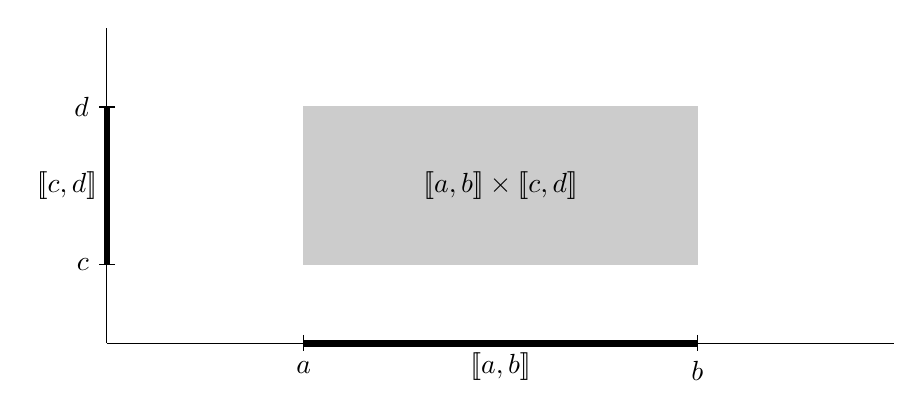
\begin{tikzpicture}[y=1cm, x=2.5cm]	
 	%axis
	\draw(0,0) -- coordinate (x axis mid) (4,0);
    	\draw (0,0) -- coordinate (y axis mid) (0,4);
    	
    	%ticks
    	\draw[fill] (1,1pt) rectangle (3,-1pt);    	
    	\draw (1, 3pt) -- (1, -3pt) node[anchor=north] {$a$};
    	\draw (3, 3pt) -- (3, -3pt) node[anchor=north] {$b$};
    	\draw (2, 0) node[anchor=north] {$[\![a,b]\!]$};
    	
    	\draw[fill] (1pt,1) rectangle (-1pt, 3);
    	\draw (3pt, 1) -- (-3pt, 1) node[anchor=east] {$c$};
    	\draw (3pt, 3) -- (-3pt, 3) node[anchor=east] {$d$};
    	\draw (0,2) node[anchor=east] {$[\![c,d]\!]$};
    	
    	\draw[fill, color=black!20] (1,1) rectangle (3,3);
    	\draw (2, 2) node {$[\![a,b]\!] \times [\![c,d]\!]$ };
\end{tikzpicture}
\end{figure}

\begin{theorem}
	The Cartesian product of a $k$-rectangle in $\mathbb{R}^m$ (where, $k\leq m$) 
	and $\ell$-rectangle in $\mathbb{R}^n$ (again, $\ell \leq n$) 
	is a $(k+\ell)$-rectangle in $\mathbb{R}^{m+n}$.
\end{theorem}

For completeness we will also define a 0-rectangle as a hybrid set containing a single point with multiplicity $1$ or $-1$.
Firstly this allows us to embed $k$-rectangles in $\mathbb{R}^n$.
For example $[\![a,b]\!] \times [\![c,d]\!] \times \hset{e^1}$ is the product of two 1-rectangles and a 0-rectangle (all over $\mathbb{R}$) and so it is a 2-rectangle over $\mathbb{R}^3$.
Specifically, it is the 2-rectangle $[\![a,b]\!] \times [\![c,d]\!]$ on the plane $z=3$.
This also illustrates the principle that given a $k$-rectangle in $\mathbb{R}^n$ where $n>k$ we can always find a $k$ dimensional subspace which also contains the rectangle.
We will re-use the interval notation from earlier although one should be careful to ``type-check'' while interpreting.
When $a$ and $b$ are real numbers then we continue to use the definition $[\![a,b]\!] = [a,b) \ominus [b,a)$.
However, when $\boldsymbol{a}$ and $\boldsymbol{b}$ are $n$-tuples (for example, coordinates in $\mathbb{R}^n$ then this is \emph{not} the oriented line interval $[\boldsymbol{a}, \boldsymbol{b}) \ominus [\boldsymbol{b}, \boldsymbol{a})$.

\begin{definition}
	Let $\boldsymbol{a} = (a_1, a_2, \ldots, a_n)$ and 
	$\boldsymbol{b} = (b_1, b_2, \ldots, b_n)$ be ordered $n$-tuples then we use the notation:
	\begin{align}
		[\![ \boldsymbol{a}, \boldsymbol{b} ]\!] 
		= [\![a_1, b_1]\!] \times [\![a_2, b_2 ]\!] \times \ldots \times [\![a_n , b_n]\!]
	\end{align}
\end{definition}

The dimension of $[\![ \boldsymbol{a}, \boldsymbol{b} ]\!]$ is equal to the number of indices where $a_i$ and $b_i$ are distinct.
For any $i$ where $a_i = b_i$, the corresponding term: $[\![ a_i, b_i ]\!]$ will be a hybrid set containing a single point, that is, a 0-rectangle.
The orientation of $[\![ \boldsymbol{a}, \boldsymbol{b} ]\!]$ is based on the number of negatively oriented intervals $[\![a_i,b_i]\!]$.
Should there be an odd number of indices $i$ such that $a_i > b_i$ then $[\![ \boldsymbol{a}, \boldsymbol{b} ]\!]$ will also be negatively oriented.
Otherwise, it will be positively oriented. 

%%%%%%%%%%%%%%%%%%%%%%%%%%%%%%%%%%%%%%%%%
%
% RIEMANN
%
%%%%%%%%%%%%%%%%%%%%%%%%%%%%%%%%%%%%%%%%%

\section{Riemann Integral on $n$-cubes}

Now that we have oriented $n$-dimensional cubes, we would like to define the integral over one.
For now, we will content ourselves with the Riemann integral and Euclidean volume.
More complex domains and other metrics will be handled in later chapters with push-backs and the Lebesgue integral.
The volume of an oriented $n$-cube in $\mathbb{R}^n$ we define to be the product of its side lengths.
Formally,

\begin{definition}
	Let $[\![\boldsymbol{a}, \boldsymbol{b}]\!]$ be a $k$-cube in $\mathbb{R}^n$ again with $\boldsymbol{a}=(a_1,\ldots, a_n)$ and $\boldsymbol{b}=(b_1,\ldots, b_n)$. 
	We denote the \textbf{volume of $\boldsymbol{[\![a,b]\!]}$} with $\text{vol}$ and define it as:
	\begin{equation}
		\text{vol}(\; [\![\boldsymbol{a}, \boldsymbol{b} ]\!] \;) = (b_1 - a_1) \cdot (b_2 - a_2) \cdot \ldots \cdot (b_n - a_n)
	\end{equation}
\end{definition}

For any $k<n$, a $k$-cube will have volume zero.
In at least one dimension, the cube will be degenerate (i.e. $a_i = b_i$) and so will contribute zero to the product.
Additionally, one can also observe that $\text{vol}( \ominus [\![\boldsymbol{a}, \boldsymbol{b} ]\!]) = - \text{vol}( [\![ \boldsymbol{a}, \boldsymbol{b} ]\!]$.


\begin{figure}[h]
\caption[Riemann Integral]{Upper and lower Riemann sums shown for the same sequence shown with light and dark rectangles respectively. A function over an oriented interval is Riemann integrable if the two sums converge.}
\centering
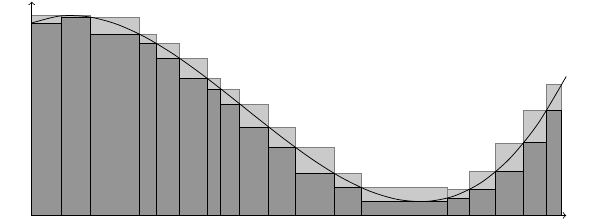
\includegraphics[scale=0.6]{diagrams/riemann}
%\begin{tikzpicture}[scale=2, domain=0:5]
%	\draw[<->] (0,2) -- (0,0) -- (5,0);
%	\draw[smooth,samples=20, domain=0.0:5.0] plot(\x, {(\x^3 - 6 * \x^2 + 4 * \x + 18)/10});
%\end{tikzpicture}
\end{figure}

Given an $n$-cube $[\![\boldsymbol{a}, \boldsymbol{b}]\!]$ we must cut each $[\![a_i, b_i]\!]$ into partitions.
Previously we used generalized partitions and did not mind if pieces overlapped or exceeded the original range.
However, for building our Riemann sums, we are only interested in partitions in the traditional, non-intersecting sense.

\begin{definition}
	Given an oriented interval $[\![a,b]\!]$ of the real line, we say that a partition of $[\![a,b]\!]$, $\{P_i\}_{i=1}^n$
	is an \textbf{interval partition of $\boldsymbol{[\![a,b]\!]}$} if its pieces are:
	\begin{enumerate}
		\item \emph{Oriented intervals}: $P_i$ is an oriented interval of the real line for all $i$.
		\item \emph{Disjoint}: $P_i \otimes P_j = \emptyset$ for all $i,j$
	\end{enumerate}
	We denote the set of all such partition as $\mathcal{P}[\![a,b]\!]$.
\end{definition}

This greatly restricts the types of partitions we have access to.
Every interval partition will be --- up to substitution of ``$]\!], (\!($'' in place of ``$)\!), [\![$'' --- of the form:
\begin{equation}
	\Big\{ \; [\![a,x_1)\!), \; [\![x_1, x_2)\!), \; [\![x_2, x_3)\!),\; \ldots,\; [\![x_{n-1}, b]\!] \; \Big\}
\end{equation}
where $x_i$ is a monotone sequence (that is, either non-increasing or non-decreasing).
This is not to say that $P_i = [\![x_{i-1}, x_i )\!)$ as the pieces of $P$ may not be given in this order.
Regardless of the ordering, we select partitions $P^j \in \mathcal{P}[\![a^j,b^j)\!)$ for each dimension of $[\![a,b)\!)$.
To build our mesh, we construct smaller $n$-cubes $I_{i_1, \ldots, i_n}$ using the Cartesian product of pieces:
\begin{equation}
	I_{i_1, \ldots, i_n} = i_1 \times \ldots \times i_n
\end{equation}
where each $i_j$ is taken from $P^j$.
We are now ready to construct Riemann sums.

\begin{definition}
	Given $P=\{ P_j \}_{j=1}^n$ where $P_j \in \mathcal{P}[\![a_j, b_j]\!]$,
	and $f:[\![\boldsymbol{a}, \boldsymbol{b}]\!] \to \mathcal{R}$ then we define a Riemann sum $f_P$ to be:
	\begin{equation}
		f_P = \sum_{i_1 \in P_1} \ldots \sum_{i_n \in P_n} f(x_{i_1, \ldots, i_n}) \text{vol}(I_{i_1, \ldots, i_n})
	\end{equation}
	where $x_{i_1, \ldots, i_n}$ is any point chosen from $I_{i_1, \ldots, i_n}$.
\end{definition}

Note that we specify \emph{a} Riemann sum, not \emph{the} Riemann sum.
There are several ways to choose $x_{i_1,\ldots,i_n} \in I_{i_1, \ldots, i_n}$ and different samplings can lead to different Riemann sums for the same partition and same function.
In $\mathbb{R}^1$, several common ways to sample include the left and right Riemann sums (which sample at the left and right boundaries), the trapezoidal Riemann sum (which averages the left and right) the upper Riemann sum (which samples at $\max(f(x_{i_1, \ldots, i_n}))$) and the lower Riemann sum (which samples at $\min(f(x_{i_1,\ldots,i_n}))$).

Recall our discussion of refinements from Chapter 2.
Given 2 partitions $P$ and $P'$ of the same set then we say $P \preceq P'$ if $P'$ is a refinement of $P$.
In this way we can induce a partial ordering on $\mathcal{P}[\![a,b]\!]$.
There is a unique smallest element in this partial ordering which is $[\![a,b]\!]$ itself; 
every partition by definition will refine $[\![a,b]\!]$.
Additionally, given $P,P' \in \mathcal{P}[\![a,b]\!]$ then propose that we can always find $Q$ that simultaneously refines both.
If $P=P'$ then trivially $Q=P$ is a common refinement.
Otherwise, we take:
\begin{equation}
	Q= [\![a,b]\!] \otimes \left( \bigoplus_{p\in P} \bigoplus_{p' \in P} p \otimes p' \right)
\end{equation}
The heavy lifting here is done by the fact that every point in $[\![a,b]\!]$ is covered by exactly one $p\in P$ and exactly one $p' \in P$.
The product of any two partition pieces will then be the smallest common interval with multiplicity 1.
Multiplying the entire thing by $[\![a,b]\!]$ is done to correct the sign.
As we go up in our ordering, our mesh becomes increasingly fine.
Taking the Riemann sum of the suprema of this poset gives us the Riemann integral.

\begin{definition}
The Riemann integral of a function $f:\mathbb{R}^n \to \mathbb{R}$ over a $k$-cube $[\![\boldsymbol{a}, \boldsymbol{b}]\!]$
where $P = \sup \Big\{ \mathcal{P} [\![a,b]\!] \Big\}$
	\begin{equation}
		\int_{[\![a,b]\!]} f(x) \; dx = f_P
	\end{equation} 
	We say that a function is \textbf{Riemann integrable} if the upper and lower Riemann sums converge.
\end{definition}


%%%%%%%%%%%%%%%%%%%%%%%%%%%%%%%%%%%%%%%%%
%
% BOUNDARY
%
%%%%%%%%%%%%%%%%%%%%%%%%%%%%%%%%%%%%%%%%%
\newpage
\section{Boundary Operator}


In one dimension, the boundary of an interval was quite straight-forward.
For a positively oriented interval, the boundary was composed of two points; 
the right end-point was positive and the left end-point was negative.
From the perspective of $k$-rectangles, 
the $\partial$ operator has mapped an oriented 1-rectangle to a set of oriented 0-rectangles.
We will now generalize the boundary to map an oriented $n$-rectangle to an $(n-1)$-rectangle.


\begin{definition}
	Let  $[\![\boldsymbol{a}, \boldsymbol{b}]\!]$ be a a $k$-rectangle in $\mathbb{R}^n$.
	Additionally, let $i_1, i_2, \ldots, i_k$ be the unique non-decreasing sequence of indices such that $a_{i_j} \neq b_{i_j}$.
	The \textbf{boundary of $ \boldsymbol{[\![ a,b ]\!]} $ }, denoted the operator $\partial$ is given by
	\begin{align}
		\partial \left( [\![ \boldsymbol{a}, \boldsymbol{b} ]\!] \right) 
		= \bigoplus_{j=1}^k (-1)^j \;
			\left(	
				[\![ 	(\boldsymbol{a}^{[\![1,n]\!]}), 
					\;\;\;
					(\boldsymbol{b}^{[\![1,i_j)\!)} 
						\oplus \boldsymbol{a}^{\hset{i_j}}
						\oplus \boldsymbol{b}^{(\!(i_j,n]\!]}) 
				]\!] \right.\;
			\notag\\
			\ominus \left.
				[\![ 	(\boldsymbol{a}^{[\![1,i_j)\!)}
						\oplus \boldsymbol{b}^{\hset{i_j}}
						\oplus \boldsymbol{a}^{(\!(i_j, n]\!]}), 
					\;\;\;		 
					(\boldsymbol{b}^{[\![1,i_j)\!)}) 			
				]\!]
			\right)
	\end{align}
\end{definition}


The above equation will require a bit of unpacking to digest featuring oriented intervals in two different contexts.
The first appears in the superscripts of $\boldsymbol{a}$ and $\boldsymbol{b}$. 
The intervals $[\![1, i_j)\!)$ and $(\!(i_j, n]\!]$ are  and is an interval over vector indices just as in Chapter 3.
Thus, the term $\boldsymbol{a}^{[\![1,i_j)\!)}$ refers to the vector $(a_1, a_2, \ldots, a_{i_j-1})$ 
while the term $\boldsymbol{b}^{(\!(i_j,n]\!]}$ refers to $(b_{i_j+1}, b_{i_j+2}, \ldots, b_{n})$.
This provides a compact notation to partition the original range of indices into 3 pieces: $[\![ 1,i_j )\!)$, $\hset{i_j}$, and $(\!(i_j, n]\!]$.
Formally, we are actually using the hybrid sets $\hset{(i_j)^1}$ but we omit multiplicity of one (and will continue to do so through out the section) to lighten notation.


Next we use the pointwise sum $\oplus$ we reconstruct $n$-dimensional vectors from our pieces.
We then construct a $(k-1)$-rectangle using these vectors as in (4.8).
Hence we will have terms of the forms:
\begin{align}
	[\![a_1, b_1]\!]
	\times \ldots \times
	[\![a_{i_{j-1}}, b_{i_{j-1}}]\!]
	\times
	[\![a_{i_j}, a_{i_j}]\!]
	\times
	[\![a_{i_{j-1}}, b_{i_{j-1}}]\!]
	\times \ldots \times
	[\![a_n, b_n]\!]
	\\
	[\![a_1, b_1]\!]
	\times \ldots \times
	[\![a_{i_{j-1}}, b_{i_{j-1}}]\!]
	\times
	[\![b_{i_j}, b_{i_j}]\!]
	\times
	[\![a_{i_{j-1}}, b_{i_{j-1}}]\!]
	\times \ldots \times
	[\![a_n, b_n]\!]
\end{align}


In each Cartesian product, the terms at $i_j$: $[\![a_{i_j}, a_{i_j}]\!]$ and $[\![b_{i_j}, b_{i_j}]\!]$ are both 0-cubes.
Since we defined the sequence $i_j$ by $a_{i_j} \neq b_{i_j}$, 
these 0-rectangles are replacing 1-cubes in $[\![\boldsymbol{a}, \boldsymbol{b}]\!]$.
Hence we are indeed left with a $(k-1)$-cube.




%%%%%%%%%%%%%%%%%%%%%%%%%%%%%%%%%%%%%%%%%
% BOUNDARY OF A 1-RECTANGLE
%%%%%%%%%%%%%%%%%%%%%%%%%%%%%%%%%%%%%%%%%
\subsection{Example: \emph{Boundary of a 1-rectangle}}
Let $\boldsymbol{a}= (a_1)$ and $\boldsymbol{b} = (b_1)$ be trivial 1-tuples. 
Then $[\![\boldsymbol{a}, \boldsymbol{b}]\!] = [\![a_1, b_1]\!]$
It follows that:
\begin{align*}
	\partial ( \; [\![ \boldsymbol{a}, \boldsymbol{b} ]\!] \; )
	=& \; (-1)^i ( [\![\boldsymbol{a}^{[\![1,1)\!)}, \boldsymbol{b}^{[\![1,1)\!)} ]\!]
	\times \hset{a_1} \times
	[\![\boldsymbol{a}^{(\!(1,1]\!]}, \boldsymbol{b}^{(\!(1,1]\!]} ]\!]\\
	&\; \ominus
	[\![\boldsymbol{a}^{[\![1,1)\!)}, \boldsymbol{b}^{[\![1,1)\!)} ]\!]
	\times \hset{b_1} \times
	[\![\boldsymbol{a}^{(\!(1,1]\!]}, \boldsymbol{b}^{(\!(1,1]\!]} ]\!] )\\
	=& \; \ominus [\![\boldsymbol{a}^{\emptyset}, \boldsymbol{b}^{\emptyset} ]\!]
	\times \hset{a_1} \times
	[\![\boldsymbol{a}^{\emptyset}, \boldsymbol{b}^{\emptyset} ]\!]\\
	& \; \oplus
	[\![\boldsymbol{a}^{\emptyset}, \boldsymbol{b}^{\emptyset} ]\!]
	\times \hset{b_1} \times
	[\![\boldsymbol{a}^{\emptyset}, \boldsymbol{b}^{\emptyset} ]\!] \\
	=& \; \hset{b_1} \ominus \hset{a_1} \\
	=& \; \hset{a^{-1}, b^{1}}
\end{align*}

One may notice a relationship between this result and the fundamental theorem of calculus:
\begin{equation}
	\int_a^b F'(x) \; dx = F(b) - F(a)
\end{equation}
Which one could easily rewrite as $\int_{[\![a,b]\!]} F'(x) \; dx = \sum (\partial([\![a,b]\!]))$.
Indeed, this is why we have defined the boundary function as such, but more general statements await.
We defined the boundary for not just intervals on $\mathbb{R}$ but $k$-cubes in $\mathbb{R}^n$.




%%%%%%%%%%%%%%%%%%%%%%%%%%%%%%%%%%%%%%%%%
% BOUNDARY OF A 3-RECTANGLE
%%%%%%%%%%%%%%%%%%%%%%%%%%%%%%%%%%%%%%%%%
\subsection{Example: \emph{Boundary of a 3-rectangle}}
Let $\boldsymbol{a} = (0,0,0)$ and $\boldsymbol{b} = (1,1,1)$.
Omitting the intermediate step, we find the boundary of $[\![ \boldsymbol{a}, \boldsymbol{b} ]\!]$ to be:
\begin{align*}
	\partial ( \; [\![ \boldsymbol{a} , \boldsymbol{b} ]\!] \; ) =
	& 	\; \ominus \; \left( \hset{0} \times [\![0,1]\!] \times [\![0,1]\!] \right)
		\; \oplus \; \left( \hset{1} \times [\![0,1]\!] \times [\![0,1]\!] \right)
	\\& 	\; \oplus \; \left( [\![0,1]\!] \times \hset{0} \times [\![0,1]\!] \right)
	 	\; \ominus \; \left( [\![0,1]\!] \times \hset{1} \times [\![0,1]\!] \right)
	\\& 	\; \ominus \; \left( [\![0,1]\!] \times [\![0,1]\!] \times \hset{0} \right)
	  	\; \oplus \; \left( [\![0,1]\!] \times [\![0,1]\!] \times \hset{1} \right)
\end{align*}

This may not be the most enlightening expression on its own.
In Figure 4.3 below, the 3-rectangle given by $[\![\boldsymbol{a}, \boldsymbol{b}]\!]$ can be seen as a cube in three dimensions.
Physically, the 3-rectangle is a solid cube and includes all interior points.
The boundary meanwhile are just the rectangular outer faces, which conveniently,
 there are also six to match the six terms of $\partial[\![\boldsymbol{a},\boldsymbol{b}]\!]$.

\begin{figure}[h]
\caption[Unit cube with boundary]{The unit cube in $\mathbb{R}^3$ with positive orientation can be represented as the 3-rectangle: $[\![(0,0,0), (1,1,1) ]\!]$ is shown as a wire-frame. 
The six faces that make up its boundary are shaded and labeled with their corresponding terms.
%Now with 100% more right-handed
}
\centering
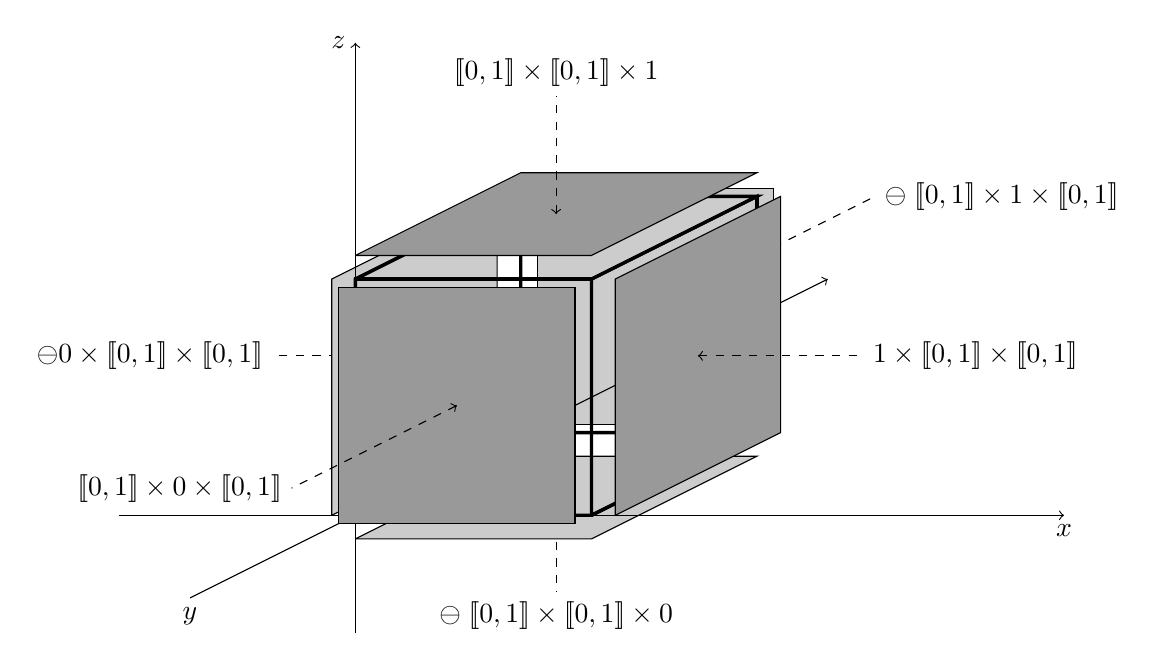
\begin{tikzpicture}[y=1.5cm, x=3cm]	
 	%axis
 	
 	%left
	\draw[color=black, dashed, <-] (0.35, 1.35) --++ (-0.7, 0) node[anchor=east, black] {$\ominus \hset{0} \times [\![0,1]\!] \times [\![0,1]\!]$};
	%back
	\draw[color=black, dashed, <-] (1.2,1.7) --++ (1,1) node[anchor=west, black] {$\ominus \; [\![0,1]\!] \times \hset{1} \times [\![0,1]\!]$};
	%bottom
	\draw[color=black, dashed, <-] (0.85,0.35) --++ (0,-1) node[anchor=north, black] {$\ominus \; [\![0,1]\!] \times [\![0,1]\!] \times \hset{0}$};
 	
 	\filldraw[fill=black!20] (0,-0.2) --++ (1,0) --++ (0.7,0.7) --++ (-1,0) --++ (-0.7,-0.7);
	\filldraw[fill=black!20] (0.77,0.77) --++ (1,0) --++ (0,2) --++ (-1,0) --++ (0, -2);
	\filldraw[fill=black!20] (-0.1,0) --++ (0,2) --++ (0.7,0.7) --++ (0,-2) --++ (-0.7,-0.7);
 	
	\draw[->] (-1,0) -- coordinate (x axis mid) (3,0) node[anchor=north] {$x$};
    	\draw[->] (0,-1) -- coordinate (y axis mid) (0,4) node[anchor=east] {$z$};
	\draw[->] (-0.7,-0.7) node[anchor=north] {$y$} --++ (2.7,2.7) ;
	
	\draw[very thick] (0,0) --++ (1,0) --++ (0.7,0.7) --++ (-1,0) --++ (-0.7,-0.7);
	\draw[very thick] (0.7,0.7) --++ (1,0) --++ (0,2) --++ (-1,0) --++ (0, -2);
	\draw[very thick] (0,0) --++ (0,2) --++ (0.7,0.7) --++ (0,-2) --++ (-0.7,-0.7);
	\draw[very thick] (0,2) --++ (1,0) --++ (0.7,0.7) --++ (-1,0) --++ (-0.7,-0.7);
	\draw[very thick] (0,0) --++ (1,0) --++ (0,2) --++ (-1,0) --++ (0, -2);
	\draw[very thick] (1,0) --++ (0,2) --++ (0.7,0.7) --++ (0,-2) --++ (-0.7,-0.7);
	
	\filldraw[fill=black!40] (0,2.2) --++ (1,0) --++ (0.7,0.7) --++ (-1,0) --++ (-0.7,-0.7);
	\filldraw[fill=black!40] (-0.07,-0.07) --++ (1,0) --++ (0,2) --++ (-1,0) --++ (0, -2);
	\filldraw[fill=black!40] (1.1,0) --++ (0,2) --++ (0.7,0.7) --++ (0,-2) --++ (-0.7,-0.7);

	%right
	\draw[color=black, dashed, <-] (1.35+0.1, 1.35) --++ (0.7, 0) node[anchor=west, black] {$\hset{1} \times [\![0,1]\!] \times [\![0,1]\!]$};
	%front
	\draw[color=black, dashed, <-] (0.5-0.07,1-0.07) --++ (-0.7,-0.7) node[anchor=east, black] {$[\![0,1]\!] \times \hset{0} \times [\![0,1]\!]$};
	%top
	\draw[color=black, dashed, <-] (0.85,2.35+0.2) --++ (0,1) node[anchor=south, black] {$[\![0,1]\!] \times [\![0,1]\!] \times \hset{1}$};
	
	
\end{tikzpicture}
\end{figure}

There are several ways to interpret and visualize the $\oplus$ and $\ominus$ sign associated with each face.
Most naturally in $\mathbb{R}^3$ for 2-rectangles is to give each a front and back side with the sign determining which to use.
Alternatively, a 2-rectangle has a boundary formed by 1-rectangles which when drawn as arrows, will all meet head-to-tail.
This induces a clockwise or counter-clockwise cycle around the edge of the rectangle and so $\circlearrowright$ and $\circlearrowleft$ are also commonly used.
This can be seen in Figure 4.4.
One may even notice that the normals produced by both are the same and choose to use that.
These are all conceptual tools, which are convenient to use particularly in $\mathbb{R}^2$ and $\mathbb{R}^3$.
There may not be such a nice physical interpretation in other spaces.


\begin{figure}[h]
\caption[Orientations of 2-rectangles]{One way of visualizing the orientation of 2-rectangles using clockwise and counter-clockwise cycles of arrows for 1-rectangles. 
The boundary of $[\![a,b]\!] \times [\![c,d]\!]$ becomes the cycle: 
$(a,c) \to (b,c) \to (b,d) \to (a,d) \to (a,c)$.
Showing the relationship between $[\![a,b]\!] \times [\![c,d]\!]$ and $[\![b,a]\!] \times [\![d,c]\!]$ }
\centering
\begin{tikzpicture}

	\def\rectCycle#1#2#3#4{
		\draw[thick, ->, color=black!80] (#1,#2) -- (#3,#2);
		\draw[thick, ->, color=black!60] (#3,#2) -- (#3,#4);
		\draw[thick, ->, color=black!40] (#3, #4) -- (#1,#4);
		\draw[thick, ->, color=black!20] (#1,#4) -- (#1,#2);
		\draw[thick, ->] (#1, 0) -- (#3, 0);
		%\draw[fill] (#1,#2) circle (1 pt);
	}

	
	\rectCycle {0+1}{1} {0+2}{2};
	\draw[<->] (0,3) -- (0,0) -- (3,0);
	\draw[very thick, ->] (0,1) -- (0,2);
	\draw (0,1.5) node[anchor=east] {$+$};
	\draw (1.5,0) node[anchor=north] {$+$};
	%\draw (1.5, 1.5) node {$+$};
	\draw(1.5,1.5) node {$\;\circlearrowleft^+$};
	
	  
	\rectCycle {4+2}{1} {4+1}{2};
	\draw[<->] (4+0,3) -- (4+0,0) -- (4+3,0);
	\draw[very thick, ->] (4+0,1) -- (4+0,2);
	\draw (4+0,1.5) node[anchor=east] {$+$};
	\draw (4+1.5,0) node[anchor=north] {$-$};
	%\draw (4+1.5, 1.5) node {$-$};
	\draw(4+1.5,1.5) node {$\;\circlearrowright^-$};
	
	
	\rectCycle {8+2}{2} {8+1}{1};
	\draw[<->] (8+0,3) -- (8+0,0) -- (8+3,0);
	\draw[very thick, ->] (8+0,2) -- (8+0,1);
	\draw (8+0,1.5) node[anchor=east] {$-$};
	\draw (8+1.5,0) node[anchor=north] {$-$};
	%\draw (8+1.5, 1.5) node {$+$};
	\draw(8+1.5,1.5) node {$\;\circlearrowleft^+$};
	
	
	\rectCycle {12+1}{2} {12+2}{1};
	\draw[<->] (12+0,3) -- (12+0,0) -- (12+3,0);
	\draw[very thick, ->] (12+0,2) -- (12+0,1);
	\draw (12+0,1.5) node[anchor=east] {$-$};
	\draw (12+1.5,0) node[anchor=north] {$+$};
	%\draw (12+1.5, 1.5) node {$-$};
	\draw(12+1.5,1.5) node {$\;\circlearrowright^-$};
	
\end{tikzpicture}
\end{figure}




%%%%%%%%%%%%%%%%%%%%%%%%%%%%%%%%%%%%%%%%%
%
% CHAINS
%
%%%%%%%%%%%%%%%%%%%%%%%%%%%%%%%%%%%%%%%%%
\section{Chains}

In fact, we have already seen $k$-chains without mentioning them explicitly.
The boundary of a $k$-cube was the sum $\oplus$, of $2k$ $(k-1)$ cubes.
Chains do not have to be boundaries however, any linear combination of $k$-cubes will do.


\begin{definition}
We denote the Abelian group of of all $k$-cubes in $X$ as $C_k(X)$ (omitting $X$ when obvious by context).
An element $c \in C_k$(X) is called a \textbf{$\boldsymbol{k}$-chain on $X$} and is of the form:
\begin{equation}
	c = \bigoplus_{c_i \in X} \lambda_i c_i
\end{equation}
with integer coefficients $\lambda_i$ and  $k$-cubes in $c_i$.
If coefficients $\lambda_i$ are $\pm 1$ and $c$ is \emph{locally finite} (i.e. each $c_i$ intersects with only finitely many $c_j$ that have non-zero coefficients) then we say that $c$ is a \textbf{domain of integration}.
\end{definition}
	
	
Since $k$-chains are just linear combinations of $k$-cubes, we naturally extend many of our definitions linearly as well.
The integral $\int_c f$ of a $k$-chain $c=\bigoplus_i \lambda_i c_i$ is defined as $\lambda_i \int_{c_i} f  + \lambda_2 \int_{c_2} f + \ldots$.
Doing the same for the boundary operator $\partial$ we have:
\begin{align*}
	&\partial_k: C_k \to C_{k-1} \\
	&\partial_k(c) = \bigoplus_{i=1}^k \lambda_i \partial_k(c_i)
\end{align*}
Elegantly, the boundary operator now maps $k$-chains to $(k-1)$-chains!
\begin{equation}
	\ldots \xleftarrow{\partial_{k-1}} C_{k-1} \xleftarrow{\partial_{k}} C_k \xleftarrow{\partial_{k+1}} C_{k+1} \xleftarrow{\partial_{k+2}} ...
\end{equation}
The most natural next question becomes \emph{``What does $\partial_{k-1}( \partial_k ( c ))$ look like?''}




%%%%%%%%%%%%%%%%%%%%%%%%%%%%%%%%%%%%%%%%%
% BOUNDARY OF A BOUNDARY
%%%%%%%%%%%%%%%%%%%%%%%%%%%%%%%%%%%%%%%%%
\subsection{Example: \emph{Boundary of a boundary (of a 2-cube)}}
Let $\boldsymbol{a} =(a_1,a_2)$ and $\boldsymbol{b}= (b_1,b_2)$.
We wish to compute $\partial_1 ( \partial_2 ( \; [\![\boldsymbol{a}, \boldsymbol{b} ]\!] \; ) )$
\begin{align}
	\partial_1 ( \partial_2 ( [\![ a_1 , b_1 ]\!] \times [\![a_2, b_2 ]\!] ) )
	=	& 	\; \ominus 	\partial_1( \hset{0} \times [\![0,1]\!]) 
			\; \oplus \; 	\partial_1(\hset{1} \times [\![0,1]\!]) \notag \\
		& 	\; \oplus 	\partial_1( [\![0,1]\!] \times \hset{0}) 
			\; \ominus \; \partial_1([\![0,1]\!] \times \hset{1}) \\
	=	& 	\ominus	( 	\ominus \hset{(0,0)} \oplus \hset{(0,1)} ) 
			\;\oplus\;(	\ominus \hset{(1,0)} \oplus \hset{(1,1)}) \notag \\
		& 	\oplus ( 		\ominus \hset{(0,0)} \oplus \hset{(1,0)} ) 
			\;\ominus\;(	\ominus \hset{(0,1)} \oplus \hset{(1,1)}) \\
	=	& \;\emptyset	
\end{align}


When moving from (4.21) to (4.22), in addition to applying $\partial_1$ we also simplify, $\hset{x} \times \hset{y} = \hset{ (x,y) }$.
The identity ``$\partial \partial = 0$'' is not unique to $2$-cubes but holds for higher dimensions as well.


\begin{figure}[h]
\caption[Boundary of a boundary (of a 2-cube)]{The boundary of 2-cube gives a cycle of oriented edges. Taking the boundary of again, at each corner, the negative boundary of one edge will be canceled by the positive boundary of the preceding edge.}
\centering
	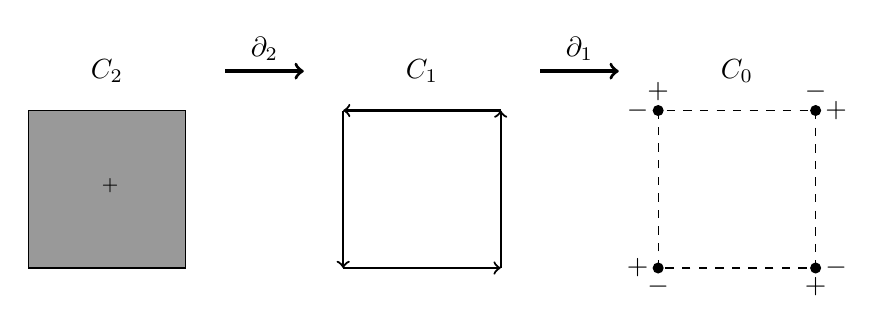
\begin{tikzpicture}
	
		\draw (1,2.5) node {$C_2$};
		\filldraw[fill=black!40] (0,0) rectangle (2,2);
		\draw (1,1) node {$\;\circlearrowleft^+$};
		
		\draw[very thick, ->] (2.5,2.5) --++ (0.5,0) node[anchor=south] {$\partial_2$} --++ (0.5,0);
		
		\draw (4+1,2.5) node {$C_1$};
		\draw[thick, ->] (4+0,0) --++ (2,0);
		\draw[thick, ->] (4+2,0) --++ (0,2);
		\draw[thick, ->] (4+2,2) --++ (-2,0);
		\draw[thick, ->] (4+0,2) --++ (0,-2);
		
		\draw[very thick, ->] (6.5,2.5) --++ (0.5,0) node[anchor=south] {$\partial_1$} --++ (0.5,0);
		
		\draw (8+1,2.5) node {$C_0$};
		\draw[dashed] (8+0,0) --++ (0,2) --++ (2,0) --++ (0,-2) --++ (-2,0);
		\fill (8,0) node[anchor=north] {$-$} node[anchor=east] {$+$} circle (2pt);
		\fill (8+2,0) node[anchor=west] {$-$} node[anchor=north] {$+$}  circle (2pt);
		\fill (8+2,2) node[anchor=south] {$-$} node[anchor=west] {$+$} circle (2pt);
		\fill (8,2) node[anchor=east] {$-$} node[anchor=south] {$+$} circle (2pt);
		
	\end{tikzpicture}
\end{figure}


Let $[\![\boldsymbol{a}, \boldsymbol{b}]\!]$ be a $k$-rectangle in $\mathbb{R}^n$.
Then we have:
\begin{align}
	\partial_k \partial_{k-1} \left( [\![ \boldsymbol{a}, \boldsymbol{b} ]\!] \right) 
	= \bigoplus_{j=1}^k (-1)^j 
		& \;  \left( \; \partial_{n-1} \left(	
			[\![ 	\boldsymbol{a}^{[\![1,n]\!]}, \;\;
				\boldsymbol{b}^{[\![1,i_j)\!)}
					\oplus \boldsymbol{a}^{[\![i_j]\!]}
					\oplus \boldsymbol{b}^{(\!(i_j,n]\!]} 
			]\!] 
		\right) \right. \notag\\[-1em]
		& \ominus \; \left. \! \partial_{n-1} \left(
			[\![ 	\boldsymbol{a}^{[\![1,i_j)\!)}
					\oplus \boldsymbol{b}^{[\![i_j]\!]}
					\oplus \boldsymbol{a}^{(\!(i_j,n]\!]} , \;\;
				\boldsymbol{b}^{[\![1,n]\!]}
			]\!] 
		\right)\right) \\[1em]
	= \bigoplus_{j=1}^k \bigoplus_{\ell=1}^{k-1} (-1)^{j+\ell}
		\;&
			[\![ 	(\boldsymbol{a}^{[\![1,n]\!]}), \;\;
				(\boldsymbol{b}^{[\![1,i_j)\!) \;\oplus\; (\!(i_j,i_{j,\ell})\!) \;\oplus\; (\!(i_{j,\ell},n]\!]}
					\oplus \boldsymbol{a}^{[\![i_j]\!] \;\oplus\; [\![i_{j,\ell}]\!]})
			]\!] \notag\\[-1em]
		\ominus \;&
			[\![ 	(\boldsymbol{a}^{[\![1,i_{j,\ell})\!) \;\oplus\; (\!(i_{j,\ell},n]\!]}
					\oplus \boldsymbol{b}^{[\![i_{j,\ell}]\!]}), \;\;
				(\boldsymbol{b}^{[\![1,i_j)\!) \;\oplus\; (\!(i_j,n]\!]}
					\oplus \boldsymbol{a}^{[\![i_j]\!]})
			]\!] \notag\\
		\ominus \; &
			[\![ 	(\boldsymbol{a}^{[\![1,i_j)\!) \;\oplus\; (\!(i_j,n]\!]}
					\oplus \boldsymbol{b}^{[\![i_j]\!]}), \;\;
				(\boldsymbol{b}^{[\![1,i_{j,\ell})\!) \;\oplus\; (\!(i_{j,\ell},n]\!]}
					\oplus \boldsymbol{a}^{[\![i_{j,\ell}]\!]})
			]\!] \notag\\
		\oplus \;&
			[\![ 	(\boldsymbol{a}^{[\![1,i_j)\!) \;\oplus\; (\!(i_j,i_{j,\ell})\!) \;\oplus\; (\!(i_{j,\ell},n]\!]}
					\oplus \boldsymbol{b}^{[\![i_j]\!] \;\oplus\; [\![i_{j,\ell}]\!]}), \;\;
				(\boldsymbol{b}^{[\![1,n]\!]})
			]\!] 
\end{align}
Note that we have $i_j$ and $i'_\ell$; after applying the first boundary operator, one dimension of the $k$-cube is degenerate.
Hence for each sequence: $\{i_j\}_{j=1}^k$ we construct $\{i_{j,\ell}\}_{\ell=1}^{k-1}$ given by:
\begin{equation}
	i_{j,1} , \ldots, i_{j,k-1} = i_1, \ldots, \widehat{i_j}, \ldots, i_k
\end{equation}
The double sum iterates over all pairs but $\oplus$ commutes so the $(k-2)$-cube with degenerate dimensions $[\![i_j]\!] \oplus [\![i_{j,\ell}]\!]$ will be iterated over twice. 
The sequences depend on one another so it is not as simple as simply swapping $\ell$ and $j$:
\begin{equation}
   [\![i_j]\!] \oplus [\![i_{j,\ell}]\!] =
     \begin{cases}
       [\![i_\ell]\!] \oplus [\![i_{\ell,j-1}]\!] & j > \ell \\
       [\![i_{\ell+1}]\!] \oplus [\![i_{\ell+1,j}]\!] & j \leq \ell
     \end{cases}
\end{equation}
So each term representing a $(k-2)$-cube will occur twice in the sum.
Once with the iteration $(j,\ell)$ and once with $(\ell, j-1)$ or $(\ell+1, j)$.
In either case, $(-1)^{j+\ell}$ is inverted meaning the two cubes will cancel.
Leaving us with the boundary of a boundary being empty.
By linearity this extends to all chains as well as the sum of empty sets is of course still empty.


\begin{definition}
	A \textbf{chain complex} is a sequence of Abelian groups $\ldots, A_2, A_1, A_0, A_{-1}, A_{-2}, \ldots$ 
	which are connected by homomorphisms $d_n:A_n \to A_{n-1}$ such that $d_n \circ d_{n+1} = 0$ for all $n$.
	Typically written out as:
	\begin{equation}
		\ldots 	\xleftarrow{d_{k-1}} A_{k-1} 
				\xleftarrow{d_{k}} A_k 
				\xleftarrow{d_{k+1}} A_{k+1} 
				\xleftarrow{d_{k+2}} \ldots
	\end{equation}
	A \textbf{cochain complex} is a sequence of Abelian groups $\ldots, A^{-2}, A^{-1}, A^0, A^{1}, A^{2}, \ldots$
	which are connected by homomorphisms $d^n:A^n \to A^{n+1}$ such that $d^n \circ d^{n-1} = 0$ for all $n$.
	Typically written out as:
	\begin{equation}
		\ldots 	\xrightarrow{d^{k-1}} A^{k-1} 
				\xrightarrow{d^{k}} A^k 
				\xrightarrow{d^{k+1}} A^{k+1} 
				\xrightarrow{d^{k+2}} \ldots
	\end{equation}
\end{definition}

$(C_\bullet, \partial_\bullet)$ is just one instance of a chain complex known as the \emph{``cubic homology''}.
In the next chapter we will look at the more general \emph{``cubic singular homology''}.
As well as the related cochain complex: the \emph{``De Rham cohomology''} and how the two relate.
















